\documentclass[a4paper,12pt]{article}
\usepackage[a4paper,top=3cm,bottom=2cm,left=3cm,right=3cm,marginparwidth=1.75cm]{geometry}
\usepackage[brazil]{babel}
\usepackage[T1]{fontenc}
\usepackage[utf8]{inputenc}
\usepackage{amsmath}
\usepackage{MnSymbol}
\usepackage{wasysym}
\usepackage{color}
\definecolor{Blue}{rgb}{0,0,0.9}
\definecolor{Red}{rgb}{0.9,0,0}
\usepackage{esvect}
\usepackage{graphicx}
\usepackage{float}
\usepackage{indentfirst}
\usepackage{caption}
\usepackage{blkarray}
\linespread{1.25}
\usepackage{pgfplots}
\usepackage{amsfonts}
\title{Relatório IC - PGDM: Um Problema Real}
\author{Guilherme Philippi; Guilherme Abreu; Ricardo E. Mueller; Lucas Pereira}
\begin{document}
	\maketitle
	\tableofcontents
	\newpage
	
	% ====================================== Grafos ========================================================
	\section{Grafos}
	\subsection{Definições Elementares}
	\noindent\textbf{Definição 1: } Um grafo $G$ é um par ordenado da forma $(V(G),E(G))$, composto por um conjunto de \textit{vértices} $V(G)$, de arestas $E(G)$ e uma \textit{função de incidência} $\psi_{g}$ que, por sua vez, associa a cada aresta de $V(G)$ um par não ordenado de vértices (nem sempre distintos) de $E(G)$. É dito que as arestas \textit{ligam} os vértices, denominados \textit{extremidades} desta aresta.
	\\
	\\
	\textbf{Definição 2: } Os números de vértices e de arestas são chamados de, respectivamente, \textit{ordem} e \textit{tamanho} de um grafo. Comumente são denotados por $v(G)$ e $e(G)$.
	\\
	\\
	\textbf{Definição 3: } As extremidades de uma aresta são denominadas \textit{incidentes} à aresta, bem como esta aresta é \textit{incidente} às \textit{extremidades}.
	\\
	\\
	\textbf{Definição 4: } Vértices distintos e incidentes à uma mesma aresta são denominados \textit{adjacentes}. Nesse sentido, arestas que possuem um vértice em comum são \textit{adjacentes} também.
	\\
	\\
	\textbf{Definição 5: } Dois vértices distintos e adjacentes são denominados \textit{vizinhos}. O conjuntos de vértices \textit{vizinhos} geralmente é denotado por $N_{G}(v)$.
	\\
	\\
	\textbf{Definição 6: } A aresta que possui o mesmo vértice como extremidades é denominada \textit{laço}.
	\\
	\\
	\textbf{Definição 7: } Uma aresta com extremidades distintas é chamada de \textit{elo}. Dois ou mais \textit{elos} com as mesmas extremidades são ditos \textit{paralelos}.
	\subsection{Tipos de Grafos}
	\noindent\textbf{Definição 8: } Um grafo é \textit{finito} se o conjunto de vértices e o conjunto de arestas forem finitos. 
	\\
	\\
	\textbf{Definição 9: } O grafo que não possui arestas e vértices é denominado \textit{grafo nulo}. Temos também que o grafo com um único vértice é chamado de \textit{grafo trivial} (todos os outros são não-triviais).
	\\
	\\
	\textbf{Definição 10: }\textit{Grafo simples} é o nome dado ao grafo que não possue laços ou arestas paralelas. \textit{Pseudografo} é o nome dado ao tipo de grafo onde são permitidos laços e arestas paralelas.
	\\
	\\
	\textbf{Exemplo 1: }Considere o grafo $G_1$ de modo que:
	\\
	\\
	$V(G_1)=\{A, B, C, D, E\}$;
	\\
	$E(G_1)=\{f,g,h,i,j,k\}$, onde, temos que $f=\{A,D\}$, $g=\{D,E\}$, $h=\{B,E\}$, $i=\{B,D\}$, $j=\{E,E\}$ e $k=\{A,D\}$. 
	\\
	\\
	\indent Veja a representação abaixo:
	\vspace{0.5cm}
	\begin{figure}[h]
		\center
		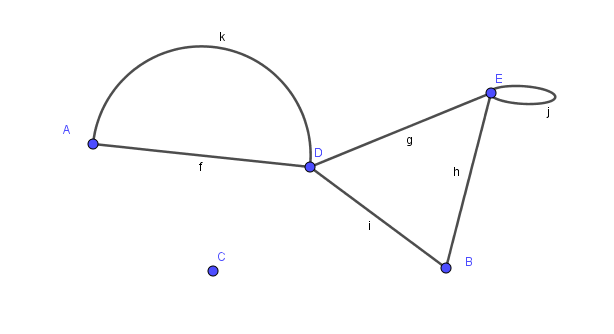
\includegraphics[width=0.8\linewidth]{Grafo1.png}
		\caption{Grafo $G_1$}
		\label{}
	\end{figure}
	\\
	\indent Inicialmente note que este grafo não é simples, pois possue arestas paralelas ($f$ e $k$) e um laço ($j$). Analisando os vizinhos dos vértices $D$ e $C$, temos que $N_G(D)=\{A,B,E\}$ e $N_G(C)=\emptyset$.
	\\
	\\
	\textbf{Definição 11: }Um grafo simples onde quaisquer dois vértices são adjacentes é denominado \textit{grafo completo}.
	\\
	\\
	\textbf{Definição 12: }\textit{Grafo conexo} é o nome dado para o tipo de grafo onde é possível estabelecer um caminho de qualquer vértice para qualquer outro vértice dele. Caso contrário, temos um \textit{grafo desconexo}. No caso extremo, temos que \textit{grafo vazio} é o grafo que não possui vértices adjacentes (não temos arestas).
	\\
	\\
	\textbf{Exemplo 2: }Note que no exemplo 1 temos um caso de grafo desconexo, pois não temos como estabelecer, por exemplo, um caminho do vértice A para o C. Abaixo segue um exemplo de grafo completo e conexo.
	\begin{figure}[h]
		\center
		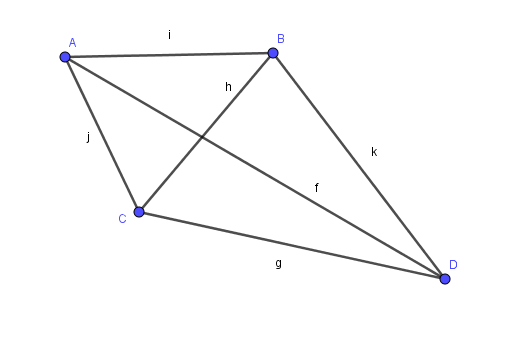
\includegraphics[width=0.6\linewidth]{Grafocompleto.png}
		\caption{Grafo Completo e Conexo}
		\label{}
	\end{figure}
	\\
	\\
	\textbf{Definição 13: }Chamamos de \textit{grafo bipartido} o grafo onde pode-se particionar o conjunto de vértices em dois, de modo que cada aresta possua extremidades em ambos os conjuntos.
	\\
	\\
	\textbf{Exemplo 3: }Um exemplo interessante de grafo bipartido é um caso análogo ao que, geralmente, utilizamos para ensinar funções. Observe a figura:
	\vspace{0.5cm}
	
	\begin{minipage}{\linewidth}% to keep image and caption on one page
		\makebox[\linewidth]{%        to center the image
			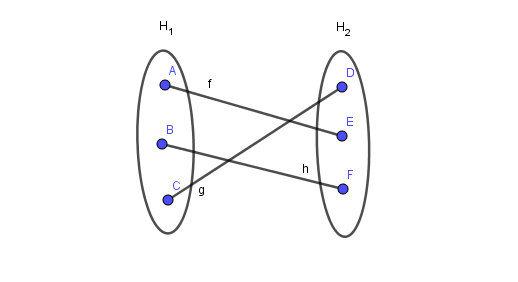
\includegraphics[keepaspectratio=true,scale=0.8]{Grafobipartido.png}}
		\captionof{figure}{Grafo Bipartido}
		\label{}%      only if needed  
	\end{minipage}
	
	%\begin{figure}[h]
	%  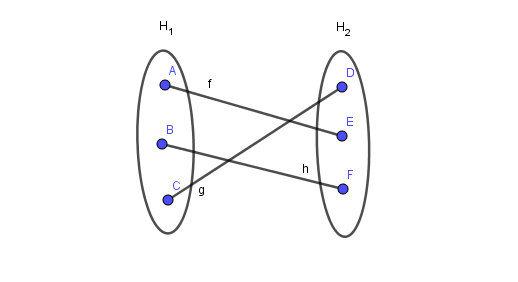
\includegraphics[width=\linewidth]{Grafobipartido.png}
	%  \caption{Grafo Bipartido}
	%  \label{}
	% \end{figure}
	\vspace{0.5cm}
	Perceba que podemos separar os vértices em dois conjuntos $H_1$ e $H_2$ de modo que cada aresta possua exatamente uma extremidade em cada conjunto.
	\\
	\\
	\textbf{\textcolor{Red}{Observação 1: }}Nem todo grafo conexo pode ser bipartido, bem como nem todo grafo bipartido é conexo. Para verificar o primeiro item basta pegarmos qualquer grafo completo com 3 ou mais vértices e, uma vez que um dos conjuntos da bipartição terá mais de 2 vértices, com certeza teremos uma aresta cujas extremidades estarão num dos conjuntos da bipartição. Pelo exemplo 3 podemos verificar o segundo item da afirmação. 
	\subsection{Subgrafos e Grafos Especiais}
	\noindent\textbf{Definição 14: }Um \textit{subgrafo} é um grafo resultante de um subconjunto de vértices e outro subconjunto de arestas de determinado grafo. No caso, deve-se destacar que todos os vértices que são extremidades de todas as arestas do escolhido subconjunto de arestas devem estar no subconjunto de vértices.
	\\
	\\
	\textbf{Exemplo 4: }Considere o grafo $G_2$, conforme ilustrado abaixo:
	\\
	\\
	\begin{figure}[h]
		\center
		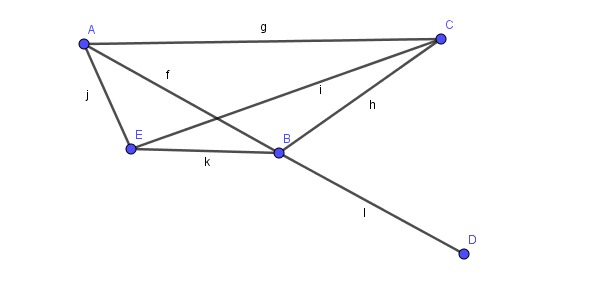
\includegraphics[width=0.6\linewidth]{Grafo2.png}
		\caption{Grafo $G_2$}
		\label{}
	\end{figure}
	\\
	\\
	Formando um subconjunto de arestas $E_s=\{i,k\}$ e de vértices $V_s=\{B,C,E\}$ obtemos o subgrafo $G_s$:
	\vspace{0.5cm}
	\begin{figure}[h]
		\center
		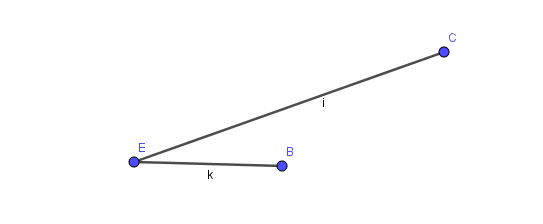
\includegraphics[width=0.6\linewidth]{subgrafo.png}
		\caption{$G_s$, subgrafo de $G_2$}
		\label{}
	\end{figure}
	\\
	\\
	\textbf{Definição 15:} \textit{Caminho} é uma sequência de vértices tal que para cada um dos vértices existe uma aresta para o vértice seguinte. Um caminho é chamado simples se nenhum dos vértices no caminho se repete. O comprimento do caminho é o número de arestas que o caminho "usa", contando-se arestas múltiplas vezes. Dois caminhos são independentes se não tiverem nenhum vértice em comum, exceto o primeiro e o último. Um caminho é $fechado$ quando começa e termina no mesmo vértice. Ao percorrer um caminho não repetimos nem vértices nem arestas.
	\\
	\\
	\textbf{\textcolor{Red}{Observação 2: }} O grafo $G_s$ é um exemplo de um caminho no grafo $G_2$. Especialmente, o grafo $G_s$ é um grafo linear, que será definido ainda.
	\\
	\\
	\textbf{Definição 16: }\textit{Caminho hamiltoniano} é um caminho onde é possível visitar cada vértice do grafo uma única vez. 
	\\
	\\
	\textbf{Exemplo 5: }Podemos estabelecer um caminho hamiltoniano no grafo $G_2$ seguindo a seguinte ordem de vértices:
	\vspace{0.5cm}
	\begin{figure}[h]
		\center
		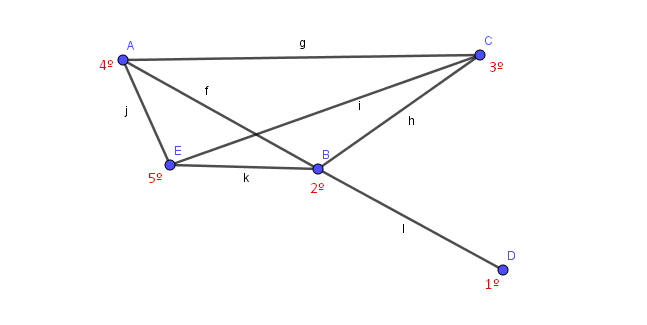
\includegraphics[width=0.6\linewidth]{hamiltoniano.png}
		\caption{Grafo $G_2$}
		\label{}
	\end{figure}
	\\
	\\
	Assim obteríamos o seguinte caminho:
	\vspace{0.5cm}
	\begin{figure}[h]
		\center
		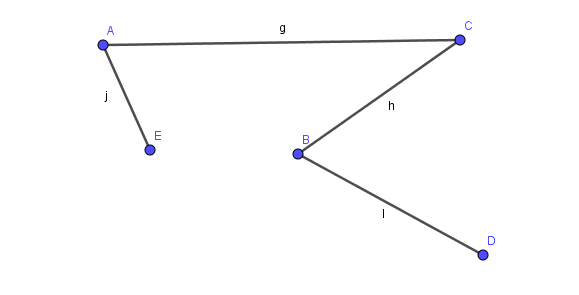
\includegraphics[width=0.6\linewidth]{hamiltoniano2.png}
		\caption{Caminho hamiltoniano de $G_2$}
		\label{}
	\end{figure}
	\\
	\\
	\textbf{Definição 17: }\textit{Caminho Euleriano} é um caminho onde cada aresta do grafo é visitada uma única vez.
	\\
	\textbf{Definição 17.1: }Um grafo é denominado \textit{atravessável} (\textit{semi-euleriano}) quando contém um caminho euleriano.
	\\
	\\
	\textbf{Exemplo 6: }Se excluirmos algumas arestas de $G_2$ obteremos o grafo interessante para o exemplo. Considere o grafo $G_e$, resultante da exclusão das arestas g, j e g de $G_2$, e reflita sobre a existência de um caminho euleriano em $G_2$:
	\vspace{1.5cm}
	\begin{figure}[h]
		\center
		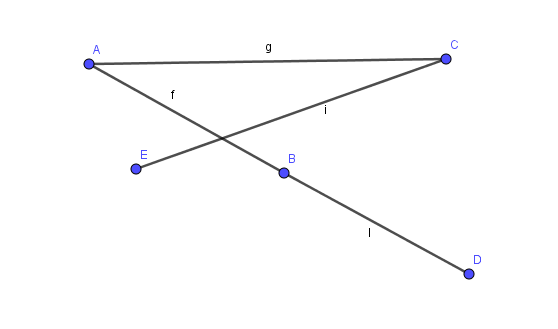
\includegraphics[width=0.7\linewidth]{caminhoeuleriano.png}
		\caption{Caminho euleriano de $G_e$}
		\label{}
	\end{figure}
	\\
	\\
	\textbf{\textcolor{Red}{Observação 3: }}Este exemplo pode não ser tão esclarecedor, devido à impossibilidade de poder se repetir vértices num caminho. Este ponto será melhor discutido na sessão intitulada Sequências de Vértices e Arestas. 
	\\
	\\
	\textbf{Definição 18: }\textit{Clique} é um subconjunto de vértices que possuem arestas entre si dois a dois. Dado um clique, caso não seja possível estender este conjunto de modo que permaneça clique, dizemos que ele é um \textit{Clique Maximal}. O clique com maior cardinalidade de um grafo $G$ é chamado de \textit{Clique Maximal de G}.
	\\
	\\
	\textbf{Exemplo 7: }Em $G_2$, um exemplo de clique seria um subgrafo $G_c$ tal que $V(G_c)=V(G_2)-\{D\}$ e $E(G_c)=E(G_2)-\{l\}$. Veja a imagem à seguir:
	\vspace{2cm}
	\begin{figure}[h]
		\center
		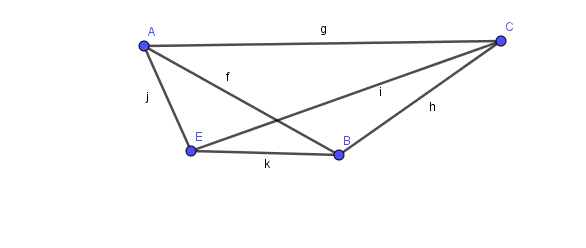
\includegraphics[width=0.6\linewidth]{cliquemaximal.png}
		\caption{Clique maximal de $G_2$}
		\label{}
	\end{figure}
	\\
	\\
	\textbf{Definição 19: }\textit{Ciclo} é um caminho em que o primeiro vértice coincide com o último. Ciclos de comprimento 1 são laços.
	\\
	\textbf{Definição 19.1: }Uma \textit{árvore} é um grafo conexo e acíclico (não contém ciclos). Uma união disjunta de árvores é denominada \textit{Floresta}.
	\\
	\\
	\textbf{Exemplo 8 : }Excluindo as arestas i e f do grafo $G_c$ obtemos um ciclo, conforme a imagem:
	\vspace{0.5cm}
	\begin{figure}[h]
		\center
		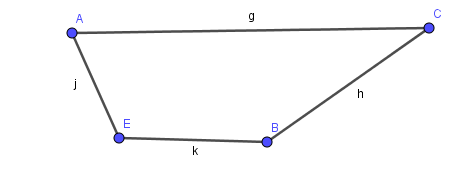
\includegraphics[width=0.6\linewidth]{circuitoeuleriano.png}
		\caption{Ciclo}
		\label{}
	\end{figure}
	\\
	\\
	\textbf{Exemplo 9: }Considere o grafo $G_3$ à seguir e perceba que se trata de uma floresta:
	\\
	\\
	\begin{figure}[h]
		\center
		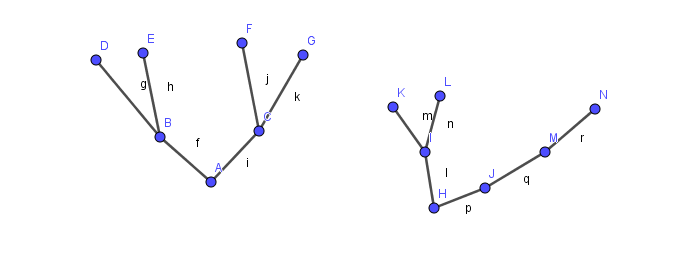
\includegraphics[width=0.7\linewidth]{floresta.png}
		\caption{Grafo $G_3$}
		\label{}
	\end{figure}
	\\
	\\
	\textbf{Definição 20: }\textit{Dígrafo (ou quiver)} é o nome dado para o grafo onde são atribuídos sentidos para cada aresta. Comumente são utilizadas setas no lugar dos segmentos para a representação.
	\\
	\\
	\textbf{Definição 21: }Chamamos de \textit{grafo ponderado} o grafo onde atribuímos valores numéricos para suas arestas.
	\subsection{Matrizes de Incidência e Adjacência}
	\noindent\textbf{Matriz de Incidência: }Cada coluna representa os vértices incidentes a determinada aresta. Assim, cada linha representa as arestas incidentes a cada vértice. Contamos 1 para aresta incidente ao vértice (ou vice-versa) e 2 se tivermos um laço. Observe a matriz de incidência de $G_1$ à seguir:
	\[
	\begin{blockarray}{ccccccc}
	f & g & h & i & j & k \\
	\begin{block}{(cccccc)c}
	1 & 0 & 0 & 0 & 0 & 1 & A \\
	0 & 0 & 1 & 1 & 0 & 0 & B \\
	0 & 0 & 0 & 0 & 0 & 0 & C \\
	1 & 1 & 0 & 1 & 0 & 1 & D \\
	0 & 1 & 1 & 0 & 2 & 0 & E \\
	\end{block}
	\end{blockarray}
	\]
	\\
	\\
	\textbf{Matriz de Adjacência: }É uma tabela onde observa-se somente a relação de adjacência entre vértices. Caso um vértice seja adjacente a outro, bota-se número 1. No caso de um laço, bota-se 2. Observe a matriz de adjacência de $G_1$:
	\[
	\begin{blockarray}{cccccc}
	A & B & C & D & E\\
	\begin{block}{(ccccc)c}
	0 & 0 & 0 & 1 & 0 & A \\
	0 & 0 & 0 & 1 & 1 & B \\
	0 & 0 & 0 & 0 & 0 & C \\
	1 & 1 & 0 & 0 & 1 & D \\
	0 & 0 & 0 & 0 & 2 & E \\
	\end{block}
	\end{blockarray}
	\]
	\subsection{Grau (ou Valência) de um Vértice}
	\noindent\textbf{Definição 22: }O \textit{grau} de um vértice é o número de arestas incidentes a ele. Cada laço conta como duas arestas. O vértice com \textit{grau} zero é chamado de \textit{vértice isolado}.
	\begin{itemize}
		\item $d_{G}(v)$: É o grau do vértice $v$. Se $G$ é um grafo simples, então $d_{G}(v)$ denota o número de vizinhos de $v$ em $G$.
		\item $\Delta(G)$: É o maior grau dentre os vértices de $G$.
		\item $\delta(G)$: É o menor grau dentre os vértices de $G$.
		\item $d(G)$: É a média de grau dos vértices de $G$.
	\end{itemize}
	\textbf{Definição 22.1: }Chamamos de \textit{Grafo Regular} aquele cujo todos os vértices possuem mesmo grau.
	\\
	\subsection*{Teorema 1: } Para todo grafo $G(V(G),E(G))$, com $m$ arestas, vale:
	\begin{equation}
	\sum\limits_{v\in V}{d(v)=2m}
	\end{equation}
	\textbf{Demonstração: }Considere a matriz de incidência M do grafo G. Para saber o grau de um determinado vértice basta olharmos para sua linha correspondente e somarmos os valores contidos na linha. Note que somar os valores presentes em todas as linhas é o mesmo que somar os valores presentes nas colunas. Como temos $m$ colunas e cada aresta possui 2 vértices incidentes, segue que $\sum\limits_{v\in V}{d(v)=2m}$.\hfill$\blacksquare$
	
	\subsection*{Teorema 2: }Em qualquer grafo o número de vértices cujo grau é ímpar, é par.
	\\
	\\
	\textbf{Demonstração: }Suponha que o número de vértices com grau ímpar seja ímpar. Note que a soma do grau de todos os vértices resulta em um número ímpar(resultado aritmético). Somando este resultado com o grau dos demais vértices, cujo grau é par, obtemos um número ímpar. Absurdo, pois $\sum\limits_{v\in V}{d(v)=2m}$. Portanto, o número de vértices cujo grau é ímpar, é par.\hfill$\blacksquare$
	
	\subsection{Sequência de Vértices e Arestas}
	Todas as definições acima foram postas em termos de uma sequência de vértices e arestas específica, denominada caminho. Entretanto, existe algo mais elementar, chamado de \textit{caminhada}. Na \textit{caminhada} podemos criar uma sequência livre de vértices e arestas, inclusive podendo repeti-los. Assim, uma melhor definição para caminho seria a de uma \textit{caminhada} onde não podem ser repetidos vértices. Além disso, temos duas outras definições derivadas da \textit{caminhada}.
	\\
	\\
	\textbf{Trilha: }É uma caminhada onde vértices podem se repetir, mas arestas não.
	\\
	\\
	\textbf{Circuito: }É uma caminhada onde o vértice inicial coincide com o final, vértices podem ser repetidos, entretanto arestas não.
	\subsection{Um aprofundamento}
	Até agora as definições foram apresentadas sem grande preocupação na utilização de linguagem matemática. Assim, à seguir seguem algumas definições com o devido rigor, e necessárias para a compreensão do problema que será apresentado nos próximos capítulos:
	\begin{enumerate}
		\item Um \textit{grafo simples não-direcionado} $G$ é um par-ordenado $(V,E)$ onde $V$ é o conjunto de vértices e $E$ um conjunto de pares não-ordenados ${u,v}$ de vértices, chamados de arestas. Para $U\subseteq V$, tome $E[U]=\{\{u,v\}\in E|u,v\in U\}$ o \textit{conjunto de arestas induzido} por U.
		\item $H=(U,F)$ é um subgrafo de $G$ se $U\subseteq V$ e $F\subseteq E[U]$. O subgrafo $H$ de $G$ é chamado de \textit{grafo induzido} por U, e denotado por $H=G[U]$ caso $F=E[U]$.
		\item O grafo $G=(V,E)$ é completo (ou um clique em $V$) se $E=\{\{u,v\} | u,v\in V\wedge u\neq v\}$.
		\item Dado o grafo $G=(V,E)$ e o vértice $v\in V$, sejam os \textit{vizinhos} de $v$ os elementos do seguinte conjunto $N_G(v)=\{u\in V | \{u,v\}\in E\}$. Além disso denotamos por $\delta_G(v)=\{\{u,w\}\in E|u=v\}$ a \textit{estrela} de $v$ em $G$. 
		\begin{figure}[H]
			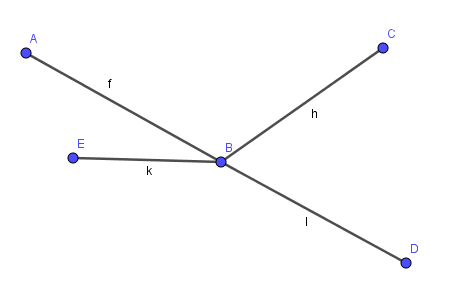
\includegraphics[width=0.6\linewidth]{estrela.png}
			\caption{Estrela de $B$ em $G_2$}
			\label{}
		\end{figure}
		\item Podemos estender a ideia de vizinhança e estrela para subconjuntos de um grafo. Dado o grafo $G=(V,E)$ e $U\subseteq V$, tomamos $N_G(U)=\bigcup_{v\in U}N_G(v)$ como a \textit{vizinhança} de $U$ e $\delta_G(U)=\bigcup_{v\in U}\delta_G(v)$ como o \textit{conjunto de corte induzido} por $U$ em $G$. Comumente usamos $N(U)$ e $\delta(U)$ também como notações. Um conjunto de corte é \textit{próprio} quando é diferente do conjunto vazio e diferente do conjunto de vértices do grafo.
		\item O grafo $G=(V,E)$ é \textit{conexo} se nenhum conjunto de corte próprio é vazio.
		\begin{figure}[H]
			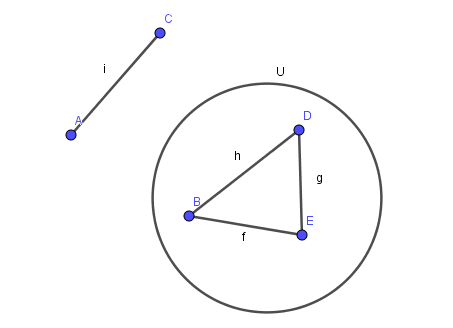
\includegraphics[width=0.6\linewidth]{desconexo.png}
			\caption{Grafo desconexo}
			\label{}
		\end{figure}
		O grafo acima é desconexo, pois podemos escolher $U=\{B,D,E\}$ e, como $U$ não possui vizinhos, segue que $N_{G_2}(U)=\emptyset$.
		\item Dado um grafo $G=(V,E)$ e $s,t\in V$, um \textit{caminho simples} H com extremos $s,t$ é um subgrafo conexo $H=(V',E')$ de $G$ de modo que $s,t \in V$, $|N_H(s)|=|N_H(t)|=1$ e $|N_H(v)|=2$ $\forall v\in V'\setminus\{s,t\}$.
		\item O grafo $G=(V,E)$ é um \textit{ciclo simples} se ele é conexo e para todo $v\in V$ temos $|N(v)|=2$.
		\item Dado um ciclo simples $C=(V',E')$ no grafo $G=(V,E)$, uma \textit{corda} de $C$ em $G$ é um par $\{u,v\}$ tal que $u,v\in V'$ e $\{u,v\}\in E\setminus E'$.
		\begin{figure}[H]
			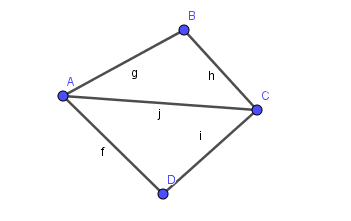
\includegraphics[width=0.6\linewidth]{corda.png}
			\caption{Ciclo com uma corda $j=\{A,C\}$}
			\label{}
		\end{figure}
		\item O grafo $G=(V,E)$ é \textit{cordal} se todo ciclo simples $C=(V',E')$ com $|E'|>3$ tem ao menos uma corda. 
		\item Dado um grafo $G=(V,E)$, $\{u,v\}\in E$ e $z\nin V$, o grafo $G'=(V',E')$ tal que $V'=(V\bigcup\{z\})\setminus \{u,v\}$ e $E'=(E\bigcup\{\{w,z\}|w\in N_G(u)\bigcup N_G(v)\})\setminus\{\{u,v\}\}$ é a \textit{contração de arestas} de $G$ em relação à $\{u,v\}$.
		\item Dado um grafo $G=(V,E)$, um \textit{pequeno grafo} de $G$ é qualquer grafo obtido de $G$ por uma repetição de contrações de arestas, eliminação de arestas e operações de eliminação de arestas.
		\item Um \textit{Grafo Molecular} é um grafo simples onde atribuímos um valor real para cada aresta. Deste modo, existe uma função $d:E\rightarrow \mathbb{R}$, que adicionamos à definição de grafo $G=(V,E,d)$.
	\end{enumerate}
	\newpage
	% ====================================== Quatérnios ========================================================
	
	\section{Quatérnios: Abordagem para um Problema Real}
	
	\subsection{A Primeira Álgebra não Comutativa}
	William Rowan Hamilton fora uma criança extremamente precoce. De origem irlandesa, viveu entre 1805 e 1865, onde, aos três anos de idade lia perfeitamente inglês. Devido a morte antecipada de seus pais teve como orientador um tio linguista e aos cinco anos sabia latim e hebraico. Até os dez anos já era familiarizado com italiano, francês, árabe, sânscrito, persa, caldeu e algumas outras línguas orientais. Ainda criança, Hamilton demonstrou grande interesse pela matemática, influenciado por autores como Newton e Laplace, caminhava a passos largos para o mundo da física e astronomia. Sem dúvidas estava florescendo um dos grandes nomes da ciência do século XIX. [9, 10]
	
	Porém, nos atentando as suas contribuições à matemática, tudo começou quando Hamilton percebeu que uma notação utilizada na teoria dos números complexos não era a mais adequada. Ele percebeu que a expressão $a + bi$ não era realmente uma soma, isto é, não é como somar dois números reais que pertencem a mesma dimensão, o que dá sentido a soma. Ele afirma que o sinal ‘$+$’ é um equívoco, um acidente histórico, e que as duas partes não podem ser naturalmente somadas. A partir deste pensamento construiu e publicou em 1833 a teoria de números complexos formalmente como conhecemos hoje, definindo a soma e produto em pares ordenados, ou seja:
	\begin{equation*}
	(a,b) + (c,d) = (a + b, c + d)
	\end{equation*}
	\begin{equation*}
	(a, b)(c, d) = (ac-bd, ad + bc)
	\end{equation*}
	
	Hamilton percebeu isso claramente pela sua inclinação física, afinal, físicos adoram se perguntar sobre as dimensões do que se está somando. Graças também a esta inclinação Hamilton logo percebeu como esta nova abordagem permitia uma visão dos números complexos como entidades orientadas no plano e, maravilhado com as possibilidades de sua descoberta, não demorou muito para que se perguntasse como seria esta relação se fosse expandida para o espaço. Infelizmente as respostas não foram fáceis e por dez anos trabalhou tentando desenvolver ternas que pudessem ser multiplicadas, tendo em vista que a soma e a subtração se davam trivialmente. A demonstração de que Hamilton nunca conseguiria sua terna encontra-se em [12]. 
	
	Até que, em 16 de outubro 1843, Hamilton, enquanto andava ao lado de sua esposa na ponte Brougham sobre o Royal Canal para presidir uma reunião do Conselho da Real Sociedade da Irlanda, dividia-se entre conversas ocasionais e no pensar sobre seu trabalho. Então teve um insight: Percebeu que seus problemas sumiriam se utilizasse quádruplas em vez de ternas e ignorasse a comutatividade para a multiplicação. Percebeu que para quádruplas $a + bi + cj + dk$ teria $i^2 = j^2 = k^2 = ijk = -1$. Desta fórmula fundamental tira-se a solução do problema da multiplicação que Hamilton encontrara, a origem da Regra de Fleming (vulgarmente conhecida como “regra da mão direita”) e, entre outras coisas surpreendentes, uma nova álgebra que iria contra os princípios matemáticos da época: \textit{A Álgebra dos Quatérnios}.
	
	\subsection{Álgebra dos Quatérnios}
	\textbf{Definição: }Seja $B_{\mathbb{R}^3}=\{i,j,k\}$ a base canônica de $\mathbb{R}^3$. Um \textit{quatérnio} é definido como um elemento da forma 
	\begin{equation}
	q=q_0+\mathbf{q_v},
	\end{equation} 
	onde $q_0 \in \mathbb{R}$ é um escalar e $\mathbf{qv}=q_1\mathbf{i}+q_2\mathbf{j}+q_3\mathbf{k}$ é um vetor de $\mathbb{R}^3$.
	\\
	
	Ou seja, todo elemento $q$ da forma $q = q_0 + q_1\textbf{i} + q_2\textbf{j} + q_3\textbf{k}$ é um quatérnio e a medida que variamos os valores dos coeficientes reais $q_0, q_1, q_2$ e $q_3$ independentemente uns dos outros na reta real percorremos todos os quatérnios possíveis, nos levando a criação do \textit{Conjunto dos Quatérnios}, definido por $\mathbb{H}$. Perceba então que há uma relação biunívoca entre $\mathbb{H}$ e $\mathbb{R}^4$, uma vez que um quatérnio pode ser escrito como a quádrupla $q = (q0, q1, q2, q3) \in \mathbb{R}^4$. [1]
	\\
	
	\textbf{Definição:} Seja $B_\mathbb{H} = \{1, \mathbf{i}, \mathbf{j}, \mathbf{k}\}$ definida como a \textit{base canônica de $\mathbb{H}$} tal que $\mathbf{i}^2 = \mathbf{j}^2 = \mathbf{k}^2 = \mathbf{ijk} = -1$.
	\\
	
	Pode-se tratar agora de operações aritméticas no Conjunto dos Quatérnios:
	\addcontentsline{toc}{subsubsection}{Operações sobre $\mathbb{H}$}
	\begin{itemize}
		\item \textbf{Adição:} dados dois quatérnios $p=p_0+\mathbf{p_v}$ e $q=q_0+\mathbf{q_v}$ em $\mathbb{H}$, define-se a adição de $p$ a $q$ como  
		\begin{equation}
		p+q=(p_0+q_0)+(\mathbf{p_v}+\mathbf{q_v})
		\end{equation}
		Temos uma proposição que mostra que esta adição está bem-definida no conjunto de quatérnios. 
		\\ \newline \textbf{Proposição:} \textit{O conjunto $\mathbb{H}$ é fechado para adição}.
		\\ \newline \textit{Demonstração.} Ou seja, o que queremos mostrar é que a soma de dois quatérnios é, por sua vez, um novo quatérnio. De fato: considerando $r=p+q$, podemos escrever o elemento $r$ como
		\begin{equation}
		r=r_0+\mathbf{r_v}
		\end{equation}
		onde sua parte escalar é dada por $r_0=p_0+q_0$ e sua parte vetorial é dada por $\mathbf{r_v=p_v+q_v}. \hfill\blacksquare$
		\\ \newline Dados $p,q,r \in \mathbb{H}$ arbitrários, temos as seguintes propriedades para a adição de quatérnios.
		\begin{enumerate}
			\item \textbf{Associatividade:} $(p+q)+r=p+(q+r)$.
			\\ \newline \textit{Demonstração.} Seja $p=p_0+\mathbf{p_v}, q=q_0+\mathbf{q_v}, r=r_0+\mathbf{r_v}$,\,\,tal que $p,q,r \in \mathbb{H}$. Partindo de $(p+q)+r$ \,\,temos:
			\\ \newline $(p+q)+r=[(p_0+\mathbf{p_v})+(q_0+\mathbf{p_v})]+(r_0+\mathbf{r_v})=[(p_0+q_0)+(\mathbf{p_v}+\mathbf{q_v})]+(r_0+\mathbf{r_v})=[(p_0+q_0+r_0)+(\mathbf{p_v}+\mathbf{q_v}+\mathbf{r_v})]=[(p_0+q_0+r_0)+(\mathbf{p_v}+\mathbf{q_v}+\mathbf{r_v})]=\{[p_0+(q_0+r_0)]+[\mathbf{p_v}+(\mathbf{q_v}+\mathbf{r_v})]\}=(p_0+\mathbf{p_v})+[(q_0+r_0)+(\mathbf{q_v}+\mathbf{r_v})]=(p_0+\mathbf{p_v})+[(q_0+\mathbf{q_v})+(r_0+\mathbf{r_v})]=p+(q+r). \hfill\blacksquare$
			\\ \item \textbf{Comutatividade:} $p+q=q+p$
			\\ \newline \textit{Demonstração.} Seja $p=p_0+\mathbf{p_v}, q=q_0+\mathbf{q_v}$,\,\,tal que $p,q \in \mathbb{H}$. Partindo de $p+q$, temos:
			\\ \newline $p+q=(p_0+\mathbf{p_v})+(q_0+\mathbf{q_v})=(p_0+q_0)+(\mathbf{p_v}+\mathbf{q_v})=(q_0+p_0)+(\mathbf{q_v}+\mathbf{p_v})=q+p.\hfill\blacksquare$
			\\ \item \textbf{Existência de Elemento Neutro:} Existe um elemento neutro, a saber, $0_{\mathbb{H}}=0_0+\mathbf{0_v} \in \mathbb{H}$, de modo que,
			\begin{equation}
			p+0_{\mathbb{H}}=0+p=p
			\end{equation}
			\\ \textit{Demonstração.}  Seja $p=p_0+\mathbf{p_v} \textrm{ e } 0_{\mathbb{H}}=0_0+\mathbf{0_v}$,\,\,tal que $p,0_{\mathbb{H}} \in \mathbb{H}$. Partindo de $p+0_{\mathbb{H}}$, temos:
			\\ \newline $p+0_{\mathbb{H}}=(p_0+\mathbf{p_v})+(0_0+\mathbf{0_v})=(p_0+0_0)+(\mathbf{p_v}+\mathbf{0_v})=(0_0+p_0)+(\mathbf{0_v}+\mathbf{p_v})=p_0+\mathbf{p_v}=p.\hfill\blacksquare$
			\\ \item \textbf{Existência de Elemento Oposto:} Existe um elemento oposto para cada $p=p_0+\mathbf{p_v} \in \mathbb{H}$, dado por $-p=-p_0-\mathbf{p_v}$, de modo que sua soma com $p$ resulte no elemento neutro da adição do item anterior, ou seja,
			\begin{equation}
			p+(-p)=(-p)+p=0_{\mathbb{H}}
			\end{equation}
			\\ \textit{Demonstração.} De fato, se partirmos de $p+(-p)$, temos:
			\\ \newline $p+(-p)= (p_0+\mathbf{p_v})+(-p_0-\mathbf{p_v})=[p_0+(-p_0)]+[\mathbf{p_v}+(\mathbf{-p_v})]=(p_0-p_0)+(\mathbf{p_v}-\mathbf{p_v})=0_0+\mathbf{0_v}=0_{\mathbb{H}}.\hfill\blacksquare$
		\end{enumerate}
		Como a adição de quatérnios satisfaz estas propriedades, temos o seguinte resultado.
		\\ \newline \textbf{Proposição: } ($\mathbb{H},+$) é um \textit{grupo abeliano}.
		\\
		
		\item \textbf{Multiplicação por Escalar:} Dado um quatérnio $q=q_0+\mathbf{q_v} \in \mathbb{H}$ e uma constante escalar real $\alpha \in \mathbb{R}$, define-se a multiplicação de $q$ pelo escalar $\alpha$ da forma
		\begin{equation}
		\alpha q=(\alpha q_0)+(\alpha \mathbf{q_v})
		\end{equation}
		A próxima proposição mostra que esta operação, unindo itens de espaços distintos, está bem definida no conjunto dos quatérnios.
		\\ \newline \textbf{Proposição:} O \textit{conjunto $\mathbb{H}$ é fechado para a multiplicação de escalares reais.}
		\\ \textit{Demonstração.} Queremos demonstrar que a multiplicação de um escalar por um quatérnio tem por resultado um novo quatérnio. Com efeito: acima, podemos considerar tal multiplicação como o elemento 
		\begin{equation*}
		r=r_0+\mathbf{r_v}
		\end{equation*}
		onde sua parte escalar é dada por $r_0=\alpha q_0 \in \mathbb{R}$ e sua parte vetorial é dada por $\mathbf{r_v}=\alpha \mathbf{q_v} \in \mathbb{R}^3.\hfill\blacksquare$
		\\ \newline A multiplicação por escalar também tem uma série de propriedades. Dados os números reais $\alpha,\beta$ e os quatérnios $p$ e $q$, temos:
		\begin{enumerate}
			\item \textbf{Associatividade:} $(\alpha \beta)q=\alpha(\beta q)$ 
			\\ \newline \textit{Demonstração.} De fato, seja $\alpha, \beta \in \mathbb{R}$ e $q=q_00+\mathbf{q_v} \in \mathbb{H}$, partindo de $(\alpha \beta)q$ temos:
			\\ \newline $(\alpha \beta)q=(\alpha \beta)(q_0+\mathbf{q_v})=\alpha \beta q_0+\alpha \beta \mathbf{q_v}=\alpha(\beta q_0+\beta \mathbf{q_v})=\alpha(\beta q).\hfill\blacksquare$
			\\ \item \textbf{Multiplicação pela Unidade:} $1q=q$
			\\ \newline \textit{Demonstração.} Queremos provar que $1q=q$. Para isto, tome $\alpha \in \mathbb{R}$, com $\alpha = 1$. Partindo de $1q=1(q_0+\mathbf{q_v})=(1q_0+1\mathbf{q_v})=q_0+\mathbf{q_v}=q$. Logo, $1q=q.\hfill\blacksquare$
			\\ \item \textbf{Distributividade em relação à soma:} estas duas propriedades unem a adição e a multiplicação por escalar e são dadas por
			\begin{equation*}
			(\alpha+\beta)q=\alpha q + \beta q
			\end{equation*}
			e 
			\begin{equation*}
			\alpha(p+q)=\alpha p + \alpha q	
			\end{equation*}
			\\ \textit{Demonstração.} Seja $\alpha,\beta \in \mathbb{R}$ e $p,q \in \mathbb{H}$.Partindo de $(\alpha + \beta)q=((\alpha + \beta)q_0 + (\alpha + \beta)\mathbf{q_v})$. Deste modo, é fácil ver que $((\alpha + \beta)q_0 + (\alpha + \beta)\mathbf{q_v})=\alpha(q_0+\mathbf{q_v})+\beta(q_0+\mathbf{q_v})=\alpha q+\beta q$. Analogamente, se olharmos para $\alpha q+\beta q$. Agora, partindo de $\alpha(p+q)=\alpha p+\alpha q$. Aplicando as devidas distributividades, temos que $\alpha p+\alpha q=(\alpha p_0+\alpha\mathbf{p_v})+(\alpha q_0+\alpha\mathbf{q_v})=\alpha p+\alpha q$. Analogamente para $\alpha p+\alpha q$. Portanto, a distributividade é válida. \hfill$\blacksquare$ 
		\end{enumerate}
	\end{itemize}
	
	Sabendo do isomorfismo já citado entre $\mathbb{H}$ e $\mathbb{R}^4$ e percebendo que as operações descritas preservam as mesmas operações entre os dois conjuntos, nota-se que existe uma relação de isomorfismo entre $\mathbb{H}$ e $\mathbb{R}^4$. Isso se deve ao fato de que o calculo vetorial como conhecemos hoje é mera simplificação das ideias de Hamilton sobre quatérnios, simplificação feita por Josiah Willard Gibbs (1839 – 1903) em um conjunto de notas para seus estudantes de física-matemática intitulado Elements of Vector Analysis [10].
	
	\textbf{Proposição:} O espaço vetorial dos quatérnios $\mathbb{H}$ é isomorfo ao espaço vetorial Euclidiano de dimensão 4, i.e. $\mathbb{H} \simeq \mathbb{R}^4$.
	\\
	
	Assim como os complexos, os quatérnios também tem conjugado. E esses são definidos da seguinte forma:
	
	\textbf{Definição:} Seja $q = q_0 + \mathbf{q_v} \in \mathbb{H}$, define-se seu \textit{conjugado} como $q^* = q_0 – \mathbf{q_v}$.
	\\
	
	Tendo as definições já estabelecidas, pode-se construir a terceira operação dos quatérnios, baseando-se em [11], justamente a que causou dez anos de trabalho para Hamilton e que torna sua álgebra um tanto não trivial, o \textit{produto algébrico dos quatérnios}:
	
	Suponha dois elementos pertencentes a $\mathbb{H}/0$, $p = p_0 + \mathbf{p_v}$ e $q = q_0 + \mathbf{q_v}$ e escritos em $B_{\mathbb{H}}$. Sabe-se que podemos escrever $\mathbf{p_v} = p_1\mathbf{i} + p_2\mathbf{j} + p_3\mathbf{k}$ e $\mathbf{q_v} = q_1\mathbf{i} + q_2\mathbf{j} + q_3\mathbf{k}$. Se multiplicarmos os dois elementos termo a termo, como na propriedade distributiva, teremos:
	\begin{equation}
	\begin{aligned}
	pq = (p_0+\mathbf{i}p_1+\mathbf{j}p_2+\mathbf{k}p_3)(q_0+\mathbf{i}q_1+\mathbf{j}q_2+\mathbf{k}q_3) \\ = (p_0q_0+p_0+\mathbf{i}p_0q_1+p_1q_0)+\mathbf{j}(p_0q_2+p_2q_0) \\ +\mathbf{k}(p_0q_3+p_3q_0)+\mathbf{i}^2p_1q_1+\mathbf{j}^2p_2q_2+\mathbf{k}^2p_3q_3+\mathbf{ij}p_1q_2+\mathbf{ji}p_2q_1 \\ +\mathbf{ik}p_1q_3+\mathbf{ki}p_3q_1+\mathbf{jk}p_2q_3+\mathbf{kj}p_3q_2
	\end{aligned}		   	       
	\end{equation}
	Mas podemos utilizar de algumas definições para simplificar a equação acima. Os produtos dos versores a seguir foram definidos por Hamilton por construção a partir de seus três planos retangulares intersectados utilizando de rotações [13].
	\begin{equation*}
	\mathbf{ij} = \mathbf{k} = \mathbf{-ji}
	\end{equation*}
	\begin{equation*}
	\mathbf{jk} = \mathbf{i} = \mathbf{-kj}
	\end{equation*}
	\begin{equation*}
	\mathbf{ki} = \mathbf{j} = \mathbf{-ik}
	\end{equation*}
	Note que esses são os produtos que fazem com que esta álgebra seja não comutativa no produto. Também são graças a esses produtos que poderemos agrupar os termos comuns em 1. Logo, usando os produtos definidos acima e a fórmula fundamental $\mathbf{i}^2 = \mathbf{j}^2 = \mathbf{k}^2 = \mathbf{ijk} = -1$ temos:
	\begin{equation}
	\begin{aligned}
	pq = (p_0q_0-p_1q_1+p_2q_2+p_3q_3)+p_0(\mathbf{i}q_1+\mathbf{j}q_2+\mathbf{k}q_3+q_0(\mathbf{i}p_1+\mathbf{j}p_2+\mathbf{k}p_3) \\ +\mathbf{i}(p_2q_3-p_3q_2)+\mathbf{j}(p_3q_1-p_1q_3)+\mathbf{k}(p_1q_2-p_2q_1).
	\end{aligned}
	\end{equation}
	Veja que conseguimos um produto interno no $\mathbb{R}^3$, uma vez que $<\mathbf{pv,qv}> = p_1q_1 + p_2q_2 + p_3q_3$, então, por uma questão de estética, para deixar está operação menor:
	\begin{equation}
	\begin{aligned}
	pq = p_0q_0-<\mathbf{pv,qv}>+p_0\mathbf{q_v}+q_0\mathbf{p_v}+\mathbf{i}(p_2p_3-p_3p_2)+\mathbf{j}(p_3q_1-p_1q_3)\\+\mathbf{k}(p_1q_2-p_2q_1)
	\end{aligned}
	\end{equation}
	Mais uma vez podemos simplificar esta equação, porém agora utilizando do produto vetorial no $\mathbb{R}^3$. Sabendo que $\mathbf{p_v} \times \mathbf{q_v} = \mathbf{i}(p_2q_3 - p_3q_2) + \mathbf{j}(p_3q_1 - p_1q_3) + \mathbf{k}(p_1q_2 - p_2q_1)$. Assim, chegamos ao produto algébrico de quatérnios, dado por:
	\begin{equation*}
	pq=p_0q_0-<\mathbf{p_v,q_v}>+p_0\mathbf{q_v}+q_0\mathbf{p_v}+\mathbf{p_v}\times\mathbf{q_v}
	\end{equation*}
	
	Agora, formalmente.
	
	\textbf{Definição} (Produto Algébrico de Quatérnios). Dados dois quatérnios não nulos $p,q \in \mathbb{H}/0$, o produto algébrico entre $p$ e $q$ é dado por 
	\begin{equation}
	pq=p_0q_0-<\mathbf{p_v,q_v}>+p_0\mathbf{q_v}+q_0\mathbf{p_v}+\mathbf{p_v}\times\mathbf{q_v}
	\end{equation}
	Considerando $p=p_0+\mathbf{p_v}$ e $q=q_0+\mathbf{q_v}$.
	
	\textbf{Proposição:} O conjunto dos quatérnios é fechado pelo produto algébrico de quatérnios.
	\\ \newline \textit{Demonstração.} De fato. Considerando a equação (11), temos que o quatérnio produto algébrico $r=pq$ pode ser escrito como 
	\begin{equation}
	r=r_0+\mathbf{r_v},
	\end{equation}
	onde $r_0=(p_0q_0-<\mathbf{p_v,q_v}>)$ e $\mathbf{r_v}=(p_0\mathbf{q_v}+q_0\mathbf{p_v}+\mathbf{p_v}\times\mathbf{q_v})$. Portanto, $r \in \mathbb{H} \hfill\blacksquare$
	\\ 
	
	\textbf{Proposição:} O produto algébrico de quatérnios é associativo. Ou seja, dados $p,q,r \in \mathbb{H}$, temos que 
	\begin{equation}
	(pq)r=p(qr)
	\end{equation}
	\\ \textbf{Proposição:} O produto algébrico de quatérnios é distributivo em relação à adição, ou seja, $p,q,r \in \mathbb{H}$
	\begin{equation}
	p(q+r)=pq+pr \,\,\,\,\,\,\,\,e\,\,\,\,\,\,\,\, (p+q)r=pr+qr
	\end{equation}
	\\
	
	Temos então o conjunto dos quatérnios monido das operações de adição, multiplicação por escalar e do produto de quatérnios, o que forma uma álgebra associativa, denominada \textit{Álgebra dos Quatérnios}. Construída tal álgebra, pode-se definir algumas propriedades interessantes.
	\\
	
	\textbf{Proposição:} Seja $1_\mathbb{H} = 1 + \mathbf{0_v} \in \mathbb{H}$ o elemento da álgebra dos quatérnios definido como identidade do produto de quatérnios. Isto é, para todo $q = q_0 + \mathbf{q_v} \in \mathbb{H}$, $q1_\mathbb{H} = q$.
	\\
	
	Como já definiu-se produto de quatérnios e conjugado, pode-se definir a norma de um quatérnio, seu tamanho:
	
	\textbf{Definição:} Dado $q \in \mathbb{H}$, sua \textit{norma} é dada por $N(q) = \sqrt[]{q^*q}$. 
	
	Duas propriedades para normas de quatérnios seguem. 
	\\
	
	\textbf{Proposição:} Dado $p \in \mathbb{H}$, a norma do conjugado de $p$ é igual a sua própria norma, ou seja, $N(p^*) = N(p)$.
	\\
	
	\textbf{Proposição:} Sejam $p, q \in \mathbb{H}$, a norma do produto $pq$ é igual ao produto das normas de $p$ e $q$, isto é, $N(pq) = N(p)N(q)$.
	\\
	
	
	
	
	% ====================================== PGDM ========================================================
	\newpage
	\section{PGDM}
	\subsection{Aspectos Históricos - Preliminares}
	Existe uma relação muito forte com a forma geométrica das moléculas orgânicas e suas funções em organismos vivos. Pode-se fazer uma analogia destes organismos com um grande quebra-cabeça, cheio de peças tão variadas quanto se queira, onde cada peça tem um local e função específica no grande quebra-cabeça, de forma que tal local e função é dado justamente pela forma geométrica de cada peça. Imagine este grande quebra-cabeça de forma tridimensional ao invés de plana, imaginando as peças com formas espaciais diversas e escalafobéticas, logo você não estará tão longe de entender como funciona um organismo vivo.
	
	Outrora, em pesquisas sobre a molécula de DNA (ácido desoxirribonucleico), descobriu-se que esse produziria um dos pilares para a vida, a proteína. Essa molécula será o alvo principal deste estudo e possuí uma gama extensa de funções em nosso organismo, como se fossem as tais peças do quebra-cabeça aludido acima. Entre tais funções, destacam-se o seu papel no transporte de oxigênio (hemoglobina), na proteção do corpo contra organismos patogênicos (anticorpos), como catalizadora de reações químicas (enzimas), receptora de membrana, atuação na contração muscular, além de outras inúmeras funções primordiais no nosso organismo [1]. Perceba a importância fundamental que tem conhecer a estrutura geométrica de cada uma dessas proteínas.
	
	Por conta dessa motivação tem-se esforços como o de Kurt Wüthrich, que propôs que se utilizasse experimentos de Ressonância Magnética Nuclear
	(RMN) para calcular a estrutura tridimensional de uma molécula de proteína, ganhando o premio Nobel da Química em 2002 [3]. Porém, a partir dessa estratégia tivemos novos problemas. A RMN não tem como resultado a estrutura tridimensional de uma proteína, mas sim distâncias entre átomos relativamente próximos que compõem a proteína. Para poder calcular a estrutura de uma proteína a partir dessas distâncias, surgira um novo problema, conhecido na literatura como Molecular Distance Geometry Problem [5].
	
	\subsection{Geometria de Distâncias}
	O principal conteúdo de estudo da Geometria de Distâncias, como o próprio nome sugere, rodeia a ideia de distância entre objetos de determinada estrutura geométrica. Assim, o problema fundamental da Geometria de Distâncias consiste em determinar um conjunto de pontos, pertencentes a um espaço geométrico, com base nas distâncias conhecidas entre tais pontos. Note que nem sempre sabemos todas as distâncias entre todos os pontos.
	\subsubsection*{Breve Histórico sobre Geometria de Distâncias}
	Temos que o surgimento da Geometria de Distâncias deu-se por volta de 1928, com o matemático Karl Menger. Entretanto, somente em 1953, com Leonard Blumenthal, que a Geometria de Distâncias tornou-se uma nova área de conhecimento.
	\\
	Por outro lado, somente em 1978, com Yemini, que o problema fundamental de Geometria de Distâncias foi enunciado. Problema onde não sabemos todas as distâncias.
	\\
	Em 1988, temos o início da utilização da Geometria de Distâncias para o cálculo de Proteínas.
	
	\subsection{Estrutura das Proteínas}
	Ao se estudar proteínas, logo se percebe sua imensidão, tanto em número como em diferenças, porém, algumas características se mantem em comum entre elas. Sabe-se que todas são formadas por aminoácidos, visto que apenas eles restam quando uma se degrada. Existem vinte tipos de aminoácidos naturais e da combinação destes por ligações petídicas formam-se todas as proteínas conhecidas. [1]
	
	Destes vinte aminoácidos, dezenove tem uma estrutura básica em comum, um carbono principal (ou também chamado, carbono alfa) ligado a um grupo amina e um grupo carboxílico. O que diferencia esses dezenove aminoácidos é o radical (ou grupo variável). Na ilustração abaixo os radicais são presentados por $R_1$ e $R_2$.
	\\
	\begin{figure}[H]
		\begin{center}
			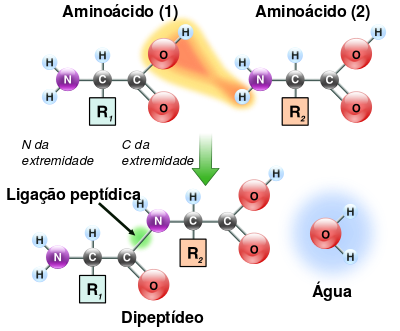
\includegraphics[width=0.6\linewidth]{Peptidformation.png}
		\end{center}
		\caption{Estrutura de um aminoácido e a síntese proteica}
		\label{}
	\end{figure}
	
	Por tanto, há uma noção prévia de qual tipo de estrutura esperar ao analisar uma molécula de proteína, isto é, existe uma ordem conhecida para as ligações dos átomos. Como as ligações atômicas vêm de processos físico-químicos, há na literatura a distância e ângulo associados a cada tipo diferente de ligação e pares de átomo. Neste problema trataremos apenas de ligações covalentes, pois há o compartilhamento de elétrons.
	
	\subsection{Representações dos Átomos em Coordenadas}
	Como as partículas que estamos interessados estão localizadas no espaço tridimensional, podemos representa-las utilizando coordenadas cartesianas tridimensionais $x_1, ...,x_n \in\mathbb{R}^3$, onde $x_n$ é a realização do n-ésimo átomo da molécula analisada. 
	
	Além da utilização das coordenadas cartesianas, também se faz uso de outro sistema de coordenadas, mais condizente com os dados que tem-se a priori da molécula, antes da solução do problema. Tal sistema denomina-se \textit{coordenadas internas}.
	
	As coordenadas internas de uma proteína são definidas pela distância entre os átomos $d_{1,2}, ..., d_{n - 1,n}$, pelo ângulo planar $\theta_{1,3}, ...,\theta_{n - 2,n}$ (formados por 3 átomos consecutivos) e pelos ângulos de torção $\omega_{1,4}, ..., \omega_{n-3,n}$ (formado por 4 átomos consecutivos). O ângulo de torção é o ângulo entre os planos formados pelos átomos $i-3,i-2,i-1$ e$i-2,i-1,i$, respectivamente. Assim, temos que $\omega$ varia no intervalo $[0,2\pi]$ e $\theta$ de $[0,\pi]$, já as distâncias entre os átomos formadas por ligações covalentes é em torno de 1,5\AA\footnote[1]{Unidade física para distâncias atômicas é o Ângstron (\AA), onde equivale a 1\AA = $10^{-10}$ m.} em vista disso só pegaremos pares de átomos tais que $d_{i,j}\leq 5 $\AA 
	\\
	
	\begin{figure}[H]
		\begin{center}
			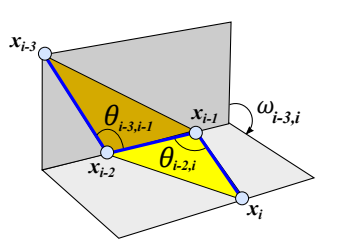
\includegraphics[width=0.6\linewidth]{Capturar.PNG}
		\end{center}
		\caption{Ângulos planos e de torção}
		\label{}
	\end{figure}
	
	Pode-se obter facilmente os ângulos planos pela \textit{Lei dos Cossenos}, tendo em vista que conhece-se todas as distâncias que, por construção, representam os lados do triângulo. Também não se encontra dificuldades para determinar os ângulos de torção, podendo utilizar da \textit{Geometria Analítica} para descobrir o ângulo entre dois vetores. Para mais detalhes, recorrer ao Apêndice A.
	
	Como trabalharemos com valores associados às distâncias entre átomos, é imprescindível a importância de se determinar as coordenadas cartesianas a partir das coordenadas internas. Isso pode ser feito pelas matrizes abaixo.
	
	Consideremos que as coordenadas do ponto $x_{i} \in\mathbb{R}^3,i= 1, ...,n $ são dadas por $(x_{i1},x_{i2},x_{i3})$, temos:
	
	$$
	\begin{bmatrix}
	x_{i1}\\ 
	x_{i2}\\ 
	x_{i3}\\ 
	1
	\end{bmatrix}
	= B_{1}B_{2}\cdots B_{i}\begin{bmatrix}
	0\\ 
	0\\ 
	0\\ 
	1
	\end{bmatrix},
	$$
	onde
	$$
	B_1\: =\:
	\begin{bmatrix}
	1 & 0 & 0 & 0\\ 
	0 & 1 & 0 & 0\\ 
	0 & 0 & 1 & 0\\ 
	0 & 0 & 0 & 1
	\end{bmatrix},\:\:\:
	\: B_2\: =\:
	\begin{bmatrix}
	-1 & 0 & 0 & -d_{1,2}\\
	0 & 1 & 0 & 0\\ 
	0 & 0 & -1 & 0\\ 
	0 & 0 & 0 & 1
	\end{bmatrix},
	$$
	$$
	B_3\:=\:
	\begin{bmatrix}
	-\cos\theta_{1,3} & -\sin\theta_{1,3} & 0 & -d_{2,3}\cos\theta_{1,3}\\ 
	\sin\theta_{1,3} & -\cos\theta_{1,3} & 0 & d_{2,3}\sin\theta_{1,3}\\ 
	0 & 0 & 1 & 0\\ 
	0 & 0 & 0 & 1
	\end{bmatrix}
	$$
	e
	$$
	B_i\:=\:
	\begin{bmatrix}
	-c_{\theta_{i}} & -s_{\theta_{i}} & 0 & -d_{i-1,i}c_{\theta_{i}}\\ 
	s_{\theta_{i}}c_{\omega_{i}} & -c_{\theta_{i}}c_{\omega_{i}}
	& -s_{\omega_{i}} & d_{i-1,i}s_{\theta_{i}}c_{\omega_{i}}\\ 
	s_{\theta_{i}}s_{\omega_{i}} & -c_{\theta_{i}}s_{\omega_{i}} & c_{\omega_{i}} & d_{i-1,i}s_{\theta_{i}}s_{\omega_{i}}\\ 
	0 & 0 & 0 & 1
	\end{bmatrix}
	$$
	onde $s_{\theta_{i}}=\sin (\theta_{i-2, i}),\: c_{\theta_{i}}=\cos (\theta_{i-2, i}),\: s_{\omega_{i}}=\sin (\omega_{i-3, i}),\: c_{\omega_{i}}=\cos (\omega_{i-3, i})$. Em $B_i$, $i=4, ..., n$.
	
	Fixando-se os comprimentos das ligações covalentes $d_{1,2},d_{2,3}$ e o valor do ângulo plano $\theta_{1,3}$, os três primeiros átomos terâo as seguintes coordenadas
	$$
	x_1\:=\:
	\begin{bmatrix}
	0\\ 
	0\\  
	0
	\end{bmatrix},\:\:\:
	x_2\:=\:
	\begin{bmatrix}
	-d_{1,2}\\ 
	0\\  
	0
	\end{bmatrix},\:\:\:
	x_3\:=\:
	\begin{bmatrix}
	-d_{1,2}+d_{2,3}\cos\theta_{1,3}\\ 
	d_{2,3}\sin\theta_{1,3}\\  
	0
	\end{bmatrix}
	$$
	
	Podemos observar que temos então uma base fixa, evitando estruturas obtidas por meio de rotações e translações a partir de uma dada estrutura.
	
	
	\subsection{RMN - Ressonância Magnética Nuclear}
	A ressonância magnética nuclear é um processo físico que analisa a interação da radiação eletromagnética com a matéria. Neste experimento é escolhida uma faixa de radiofrequência para bombardear uma amostra que está imersa em um campo magnético bastante intenso. Dependendo da radiofrequência utilizada, alguns núcleos atômicos irão absorver energia e outros não. Caso atinja-se uma frequência exata de ressonância dentro destes núcleos atômicos, é possível medir essa ressonância como um sinal de radiofrequência enviado dos núcleos atômicos. No PGDM, a frequência utilizada é para a ressonância dos núcleos de hidrogênio e um computador capta essas respostas eletromagnéticas dos núcleos atômicos para utilizar como dados do problema. [6]
	
	Assim, esse procedimento fornece vários \textit{intervalos} de distâncias possíveis relativas associadas a átomos de hidrogênio próximos (sendo que as vezes também consegue captar átomos de um isótopo específico de carbono, devido a proximidade da frequência), esses intervalos também são chamados de \textit{distancias intervalares}. Pode-se representar essas distancias intervalares matematicamente por intervalos de números reais $[d_{i,j}^i, d_{i,j}^f]$ . Isto é, existe um real $d_{i,j}$ que representa a distância real tal que
	
	$$ 0 \leq d_{i,j}^i \leq d_{i,j} \leq d_{i,j}^f$$
	
	\subsection{Modelagem Matemática}
	Quando um cientista de outra área se depara com um problema que não consegue resolver e precisa recorrer aos matemáticos, quase sempre se torna uma tarefa muito complicada para quem for tentar desenvolver o problema. Não pela complexidade matemática do assunto, isto os matemáticos dominam. A dificuldade está em entender o problema de outras áreas e, como se por ironia, resolve-los. Este é um fardo que se tem de carregar quando se escolhe trabalhar com uma ciência que é utilizada por tantas outras. No entanto, por sorte, os matemáticos são apaixonados por interpretar, modelar e resolver problemas.
	
	A boa interpretação de um problema de matemática aplicada deve se ater a algumas perguntas importantes:
	\begin{itemize}
		\item \textbf{Quais são as hipóteses?} Ou seja, fatos dos quais devemos nos basear e nos limitar para propor, de forma dialética, uma solução para o problema. Nos importaremos com seis hipóteses que advém de informações já discutidas aqui:
		\begin{description}
			\item[Hipótese 1:]as distâncias fornecidas pelos experimentos de RMN estão associados a pares de átomos conhecidos: nós sabemos a quais átomos as distâncias se referem (isso não é bem verdade, mas supomos que seja assim para desenvolver o problema);
			\item[Hipótese 2:]todos os átomos da molécula da proteína cuja estrutura 3D queremos calcular são conhecidos: conhecermos a estrutura química da molécula;
			\item[Hipótese 3:]todos os átomos da molécula de proteína estão ligadas a algum átomo, cuja distância é conhecida: não há átomos soltos, afinal, se existisse, seria outra molécula;
			\item[Hipótese 4:]existe uma ordem, dada a priori, entres os átomos da cadeia principal da proteína cuja estrutura 3D queremos calcular: conhecemos o esqueleto padrão, formado de aminoácidos, da molécula de proteína examinada;
			\item[Hipótese 5:]as distâncias entre os átomos de uma molécula de proteína separados por duas ligações covalentes são conhecidas: existem esses resultados na literatura;
			\item[Hipótese 6:]as distâncias fornecidas pela RMN são representandos por intervalos de números reais que contêm o valor correto associado.
		\end{description}
		
		\item \textbf{Qual resultado deseja-se obter?} De forma simplificada, qual é nossa \textit{tese}? Dificilmente se chega no lugar ideal se não há o conhecimento da direção a seguir. Cabe-se uma definição formal dos nossos objetivos:
		
		\textit{Deve-se determinar os pontos} $x_{i}\in\mathbb{R}^3$, \textit{i = 1, ..., n (n é o número de átomos da molécula), satisfazendo as equações}
		$$\|x_i -x_j\|=d_ij , \forall\in E
		$$
		\textit{onde} $E \subset \{1, ...,n\} \times \{1, ...,n\}$ e $d_{ij}$ \textit{são os valores de distâncias fornecidas pela RMN.}
		
		Tentar resolver os sistemas de equações acima parece não ser uma boa ideia, já que existem evidências de que não seja possível obter uma fórmula fechada para isso [2]. Podemos até tentar resolver numericamente, porém as soluções seriam infinitas para as equações.
		
		A abordagem mais usual é a representação do problema usando otimização. Para isso devemos  resolver todas as equações do problema. Podemos, dessa maneira, considerar uma única expressão com todas elas, dada por
		$$ f(x_1, ...,x_n) \equal \sum_{(i,j) \in E} (\|x_i - x_j\| - d_{ij})^2
		$$
		
		Para resolvermos tal otimização, basta encontrar valores de $x_i \in \mathbb{R}^3$, $i = 1, ..., n$, tal que $f(x_1, ...,x_n)=0.$ Assim temos
		$$ \min_{x_t \in\mathbb{R}^n} f(x_1, ...,x_n).
		$$
		
		A dificuldade nesse caso está em encontrar o mínimo global, pois existem vários mínimos locais e estes\textit{ crescem exponencialmente com a  quantidade de átomos da molécula}. Outro ponto delicado, é complicado distinguir mínimo local de global, uma vez que os métodos de otimização continua só se referem a informações locais. Isso tudo torna o problema muito custoso para resolver.
	\end{itemize}
	
	\subsubsection*{Problema de Geometria de Distâncias Moleculares: Uma definição formal}
	Agora que temos uma boa base, vamos definir o Problema de Geometria de Distâncias Moleculares formalmente utilizando grafos.
	\\
	
	Dado um grafo simples não-direcionado $G=(V,E)$, de modo que suas arestas sejam valoradas por uma função não-negativa $d:E\rightarrow\mathbb{R_+}$, considere a seguinte aplicação:
	$$x:V\rightarrow\mathbb{R}^3
	$$
	De modo que para todo $\{u,v\}\in E$ temos:
	$$\|x(u)-x(v)\|=d({u,v})
	$$
	Logo, nossa tarefa é encontrar uma aplicação $x$ que satisfaça todas as distâncias e dados do grafo que temos. Esta função é denominada \textit{realização} de $G$. Quando a realização satisfaz todas as equações da forma "$\|x(u)-x(v)\|=d({u,v})$", dizemos que ela é uma \textit{realização válida}.
	
	
	\subsection{Modelagem Computacional}
	
	Uma vez que existe uma introdução a modelagem matemática do problema, pode-se pensar em uma abordagem computacional. Não é segredo para ninguém que a computação veio e vem melhorando muito a forma como se faz matemática, introduzindo novas ferramentas e campus de estudo de grande importância. Vamos utilizar dessa evolução para a solução desse problema que, de outra forma, não seria viável. Na verdade, um dos estudos que estamos despostos a fazer aqui é se, mesmo com toda nossa capacidade computacional atual, o problema tem uma solução viável. Definiremos melhor adiante o que é uma solução dita \textit{viável}. 
	
	\subsubsection*{Dados de Entrada e Saída}
	É costume de programação se preocupar em deixar claro quais dados devem ser de entrada (\textit{input}), para serem utilizados, processados, modificados e todo o resto que necessitar para gerar os dados de saída (\textit{output}).
	
	Existem dois tipos de dados que serão tratados aqui, os dados \textit{teóricos} e os dados \textit{reais}. Todos os dados reais que utilizamos são provenientes dos experimentos de RMN. Já os teóricos vem de conhecimento da Química, Física e Biologia.
	
	\begin{description}
		\item{Dados de Entrada:}
		\begin{itemize}
			\item quantidade de átomos: $n$;
			\item sequências de átomos:
			$$N^1,C^{1}_{\alpha},C^1,N^2,C^{2}_{\alpha},C^2, ...,N^{n/3},C^{n/3}_{\alpha},C^{n/3};
			$$
			\item distância entre os átomos separados por uma ligação covalente: $\{d_{1,2},d_{2,3}, ...,d_{n-1,n}\}$, onde $i = 2, ..., n;$
			\item distância entre os átomos separados por duas ligações covalentes: $\{d_{1,3},d_{2,4}, ...,d_{n-2,n}\}$, $i=3, ..., n;$
			\item distância entre átomos próximos, com no máximo 5 \AA, fornecidas pela RMN \textit{- único dado de entrada real};
		\end{itemize}
		\item{Dados de Saída:}
		\begin{itemize}
			\item posições $x_1, ...,x_n \in\mathbb{R}^3$ dos $n$ átomos da proteína.
		\end{itemize}
	\end{description}
	
	Como as distâncias fornecidas pela RMN são um dado real, não são um valor exato. Dados reais são incertos, dependem de muitas variáveis, como a precisão da ferramenta que a mediu, o tipo de medida, quantas vezes fora medido, entre outras coisas. Esta incerteza é calculada e pode-se saber mais sobre em [7].
	
	\subsubsection*{Complexidade do PGDM}
	É de extrema importância verificarmos o curso computacional de se tentar resolver o PGDM, pois, só com esta analise, pode-se dizer se o problema tem ou não uma solução viável. Caso não tenha, o trabalho pode ser encerrado por aqui. De nada nos adianta solução que não pode ser calculada.
	
	Para poder calcular o custo computacional de uma solução matemática, deve-se verificar quantas vezes o \textit{núcleo} do programa é computado, ou seja, se verifica quantas vezes a operação central do programa é realizada. Caso for realizada apernas uma vez, dizemos que o custo é baixo. Caso essa quantidade cressa proporcionalmente a medida que aumentamos os dados de entrada do problema (por exemplo, a medida que aumentamos a quantidade $n$ de átomos da molécula), então dizemos que a dificuldade é linear. Para mais detalhes sobre custo computacional, leia [8]. Resolvemos, então, um PGDM simples e verificamos qual seria seu custo.
	
	Considere um PGDM restrito ao plano, onde temos um grafo $G = (V(G), E(G))$ tal que $V(G)=\{u, v, r, s\}$ e $E(G)=\{\{u,v\}, \{u, r\}, \{v, r\}, \{v, s\}, \{r, s\}, \{u, s\}\}$. Fixando \textit{u, v, r} e \textit{s}, ou seja, determinando $ x_{u}, x_{v},x_{r} \in\mathbb{R}^2$ de tal modo que $\|x_{u} - x_{v}\|= d_{uv}$,  $\|x_{u} - x_{r}\|= d_{ur}$ e $\|x_{v} - x_{r}\|= d_{vr}$, podemos montar o  seguinte sistema quadrático:
	$$ \|x_{s} - x_{u}\|= d_{us} $$$$ \|x_{s} - x_{v}\|= d_{vs} $$$$ \|x_{s} - x_{r}\|= d_{rs} $$
	Elevando os termos ao quadrado,
	$$\|x_{s}\|^{2} - 2(x_{s}.x_{u}) + \|x_{u}\|^{2} = d_{us}^{2}$$
	$$\|x_{s}\|^{2} - 2(x_{s}.x_{v}) + \|x_{v}\|^{2} = d_{vs}^{2}$$
	$$\|x_{s}\|^{2} - 2(x_{s}.x_{r}) + \|x_{r}\|^{2} = d_{rs}^{2}$$
	subtraindo a primeira equação das outras duas, temos:
	$$2(x_{s}.x_{v}) - 2(x_{s}.x_{u}) = \|x_{v}\|^{2} - \|x_{u}\|^{2} + d_{us}^{2} - d_{vs}^{2}$$
	$$2(x_{s}.x_{r}) - 2(x_{s}.x_{u}) = \|x_{r}\|^{2} - \|x_{u}\|^{2} + d_{us}^{2} - d_{rs}^{2}$$
	Colocando $x_{s}$ em evidência para ficar claro as incógnitas
	$$2(x_{v} - x_{u})x_{s} = \|x_{v}\|^{2} - \|x_{u}\|^{2} + d_{us}^{2} - d_{vs}^{2}$$
	$$2(x_{r} - x_{u})x_{s} = \|x_{r}\|^{2} - \|x_{u}\|^{2} + d_{us}^{2} - d_{rs}^{2}$$
	Por tanto, temos um sistema linear $Ax = b$, onde
	$$
	A = 2\begin{bmatrix}
	x_{v1} - x_{u1} & x_{v2} - x_{u2}\\
	x_{r1} - x_{u1} & x_{r2} - x_{u2}
	\end{bmatrix},
	$$
	$$
	b = \begin{bmatrix}
	\|x_{v}\|^{2} - \|x_{u}\|^{2} + d_{us}^{2} - d_{vs}^{2}\\
	\|x_{r}\|^{2} - \|x_{u}\|^{2} + d_{us}^{2} - d_{rs}^{2}
	\end{bmatrix},
	$$
	e
	$$
	x = \begin{bmatrix}
	x_{s1}\\
	x_{s2}
	\end{bmatrix}.
	$$
	
	Se a matriz \textit{A} for inversível, temos uma única solução $x^{*} = A^{-1}b$. Logo, podemos concluir que se o grafo \textit{G} de um PGDM for completo, podemos resolver o problema através da resolução de $n$ sistemas lineares, sendo $n$ proporcional ao número de vértices (átomos da molécula). Diz-se, então, que o problema pode ser resolvido em tempo \textit{linear}.
	
	No entanto, isso não acontece. Sabemos que o grafo molecular não é completo pois algumas distâncias não são informadas, assim, teremos apenas parte do grafo. 
	
	Admitindo que todas as distâncias dadas são valores \textit{precisos} e que certamente representam as distâncias entre os átomos, o problema então terá uma solução. Para encontrarmos a solução devemos achar o mínimo global discutido na modelagem matemática, que, como vimos anteriormente, é inviável. A quantidade de mínimos locais cresce exponencialmente com a quantidade de vértices. Ou seja, o custo computacional para resolver um PGDM onde, suponha, todas as distâncias da RMN são realmente precisas, pode ser proporcional a $2^n$, onde $n$ é a quantidade de átomos. O que faz esse problema entrar na classificação \textit{NP-difícil}. [8]
	\\
	\subsection{Número de soluções de um PGDM}
	Com base no que temos, podemos analisar condições para garantir a finitude do conjunto solução do PGDM. A cardinalidade do conjunto solução de um PGDM (elementos são funções) pode ajudar na solução do problema. Sabemos que um PGDM pode ter conjunto solução vazio, solução única ou ser não-enumerável. Para essa analise, consideremos o mesmo problema da seção anterior, porém, nesse caso, os vértices não estão restritos ao plano. Temos, então, um PGDM com $V=\{u, v, r, s\}$ e $E=\{\{u,v\}, \{u, r\}, \{v, r\}, \{v, s\}, \{r, s\}, \{u, s\}\}$. Fixamos \textit{u, v, r} e \textit{s}, obtemos o mesmo sistema quadrático:
	$$
	\|x_{s} - x_{u}\|= d_{us}
	$$
	$$
	\|x_{s} - x_{v}\|= d_{vs}
	$$
	$$
	\|x_{s} - x_{r}\|= d_{rs}
	$$
	Fazendo o mesmo procedimento anterior de elevar ao quadrado e subtrair a primeira das outras duas, obtemos:
	$$
	2(x_{v} - x_{u})x_{s} = \|x_{v}\|^{2} - \|x_{u}\|^{2} + d_{us}^{2} - d_{vs}^{2}
	$$
	$$
	2(x_{r} - x_{u})x_{s} = \|x_{r}\|^{2} - \|x_{u}\|^{2} + d_{us}^{2} - d_{rs}^{2}
	$$
	Até agora, nada mudou, porém, agora escrevendo explicitamente, temos:
	$$
	\begin{bmatrix}
	x_{v1} - x_{u1} & x_{v2} - x_{u2} & x_{v3} - x_{u3}\\
	x_{r1} - x_{u1} & x_{r2} - x_{u2} & x_{r3} - x_{u3}
	\end{bmatrix}
	\begin{bmatrix}
	x_{s1}\\
	x_{s2}\\
	x_{s3}
	\end{bmatrix} =
	\frac{1}{2}\begin{bmatrix}
	\|x_{v}\|^{2} - \|x_{u}\|^{2} + d_{us}^{2} - d_{vs}^{2}\\
	\|x_{r}\|^{2} - \|x_{u}\|^{2} + d_{us}^{2} - d_{rs}^{2}
	\end{bmatrix}
	$$
	Ou seja, não temos mais uma matriz $2 \times 2$, mas  sim, uma matriz $2 \times 3$.
	
	Reescrevendo o sistema de outra maneira
	$$
	\begin{bmatrix}
	x_{s1}\\
	x_{s2}
	\end{bmatrix} +
	\begin{bmatrix}
	x_{v3} - x_{u3}\\
	x_{r3} - x_{u3}
	\end{bmatrix}
	\begin{bmatrix}
	x_{s3}
	\end{bmatrix} =
	\frac{1}{2} \begin{bmatrix}
	\|x_{v}\|^{2} - \|x_{u}\|^{2} + d_{us}^{2} - d_{vs}^{2}\\
	\|x_{r}\|^{2} - \|x_{u}\|^{2} + d_{us}^{2} - d_{rs}^{2}
	\end{bmatrix}
	$$
	E supondo que a matriz
	$$
	A = \begin{bmatrix}
	x_{v1} - x_{u1} & x_{v2} - x_{u2}\\
	x_{r1} - x_{u1} & x_{r2} - x_{u2}
	\end{bmatrix}
	$$
	seja inversível, obtemos
	$$
	\begin{bmatrix}
	x_{s1}\\
	x_{s2}
	\end{bmatrix} =
	\frac{1}{2} A^{-1} \begin{bmatrix}
	\|x_{v}\|^{2} - \|x_{u}\|^{2} + d_{us}^{2} - d_{vs}^{2}\\
	\|x_{r}\|^{2} - \|x_{u}\|^{2} + d_{us}^{2} - d_{rs}^{2}
	\end{bmatrix} -
	A^{-1}\begin{bmatrix}
	x_{v3} - x_{u3}\\
	x_{r3} - x_{u3}
	\end{bmatrix}
	\begin{bmatrix}
	x_{s3}
	\end{bmatrix}
	$$
	isso agora implica que não temos mais solução, pois, para cada valor de $x_{s3} \in\mathbb{R}$, obtemos valores para $x_{s1}$ e $x_{s2}$.
	
	Para encontramos uma solução, devemos retornar ao sistema quadrático e resolver uma equação do sistema linear acima.
	
	Geometricamnete, temos a intersecção de uma reta, dada por
	$$
	\begin{bmatrix}
	x_{s1}\\
	x_{s2}
	\end{bmatrix} =
	A -
	B
	\begin{bmatrix}
	x_{s3}
	\end{bmatrix}
	$$
	onde
	$$
	A = \frac{1}{2} \begin{bmatrix}
	x_{v1} - x_{u1} & x_{v2} - x_{u2}\\
	x_{r1} - x_{u1} & x_{r2} - x_{u2}
	\end{bmatrix}^{-1} 
	\begin{bmatrix}
	\|x_{v}\|^{2} - \|x_{u}\|^{2} + d_{us}^{2} - d_{vs}^{2}\\
	\|x_{r}\|^{2} - \|x_{u}\|^{2} + d_{us}^{2} - d_{rs}^{2}
	\end{bmatrix} 
	$$
	$$
	B = \begin{bmatrix}
	x_{v1} - x_{u1} & x_{v2} - x_{u2}\\
	x_{r1} - x_{u1} & x_{r2} - x_{u2}
	\end{bmatrix}^{-1}
	\begin{bmatrix}
	x_{v3} - x_{u3}\\
	x_{r3} - x_{u3}
	\end{bmatrix}
	\begin{bmatrix}
	x_{s3}
	\end{bmatrix}
	$$
	e uma esfera tal que
	$$
	\|x_{s} - x_{u}\|= d_{us}
	$$
	resultando em 3 possibilidades: conjunto vazio (a reta não intersepta a esfera), apenas um ponto (a reta é tangente à esfera), dois pontos (a reta é secante à esfera).
	
	A discussão sugere dois aspectos importantes sobre a finitude:
	
	\begin{enumerate}
		\item Para cada vértice $s\in V$ a ser realizado em $\mathbb{R}$, devem existir arestas ${u, s}, {v, s}, {r, s} \in E$ tais que os vértices $u, v, r \in V$ já tenham sido realizados, para que se possa gerar um sistema quadrático, com $x_{s} \in\mathbb{R}^{3}$ como única incógnita, dado por
		$$
		\|x_{s} - x_{u}\|= d_{us}
		$$
		$$
		\|x_{s} - x_{v}\|= d_{vs}
		$$
		$$
		\|x_{s} - x_{r}\|= d_{rs}
		$$
		\item Para que esse sistema tenha no máximo duas soluções, a matriz linear do sistema obtido subtraindo uma equação das outras duas deve ter posto completo.
	\end{enumerate}
	
	As duas informações cruciais, relacionadas ao vértice $s\in V$, são:
	\begin{itemize}
		\item Existem $u, v, r \in V$ tais que ${u, s}, {v, s}, {r, s}\subset E$,
		\item $x_{u}, x_{v}, x_{r} \in\mathbb{R}^{3}$ fazem parte de uma realização \textit{parcial} válida. 
	\end{itemize}
	
	A ideia que conecta os pontos anteriores está ligada ao conceito de \textit{ordem nos grafos} do grafo $G = (V, E, d)$ do PGDM. Se existir uma ordem dos vértices que satifaz as condições 1 e 2 acima, podemos garntir, a menos de rotações e translações, que o cojunto solução do problema é finito.
	
	Relembremos que resolver um PGDM é conseguir uma realização válida $x: V \rightarrow\mathbb{R}^{3}$ do grafo associado, o que implica, por sua vez, definir um ponto $x_{s}\in\mathbb{R}^3$, para cada $s\in V$, satisfazendo todas as equações do sistema
	$$
	\forall {u, v}\in E, \|x_{u} - x_{v}\| = d_{uv}.
	$$
	Portanto uma solução do problema pode ser representada, então, como um elemento do $\mathbb{R}^{3\|V\|}$
	\\
	\newpage
	\section*{Referências}
	[1]  Fidalgo, Felipe Delfini Caetano, Dividindo e conquistando com simetrias em geometria de distâncias / Felipe Delfini Caetano Fidalgo. - Campinas, SP : [s.n.], 2015.
	\\
	
	[2]  C. Lavor, N. Maculan, M. Souza, R. Alves, Álgebra e geometria no cálculo de estrutura moleculares, 31º Colóquio Brasileiro de Matemática, IMPA, 2017.
	\\
	
	[3] K. W¨utrich, Protein structure determination in solution by nuclearmagnetic resonance spectroscopy, Science, 243 (1989), 45-50.
	\\
	
	[4]  Alfredo Steinbruch e Paulo Winterle. Geometria Analítica. Makron Books, São Paulo, 2a. edição, 1987.
	\\
	
	[5] L. Liberti, C. Lavor, N. Maculan, A. Mucherino, Euclidean distance geometry and applications, SIAM Review, 56 (2014), 3–69.
	\\
	
	[6] TRTF/EMRF: The history of MRI (Peter A. Rinck, ed). url = http://www.magnetic-resonance.org/ch/20-01.html
	\\
	
	[7] Tratamento estatistico de dados em fisica experimental - livro que tenho que ver na ufsc depois, relevar
	\\
	
	[8] Custo computacional, teoria da computação - mesmo caso da referencia acima
	\\
	
	[9] BOYER, Carl Benjamin. História da matemática. São Paulo: Edgard Blücher/EDUSP, 1974.
	\\
	
	[10] MILIES, P. C. Breve história da álgebra abstrata, Disponível em http://www.aguaforte. com/antropologia/cidade.htm. Acesso em nov. 2015
	\\
	
	[11] J. B. Kuipers. Quaternions and Rotation Sequences. Princeton University Press, Princeton, New Jersey, 1999. 
	\\
	
	[12] Álgebra de Quatérnios - Jucineide Silva Santos e Maurício de Araujo Ferreira, August 22, 2011
	\\
	
	[13] HAMILTON, W. R, Elements of Quaternions – Book II pag 156 %: https://books.google.com.br/books?hl=pt-
	%BR&lr=&id=hIRLX0PNxiMC&oi=fnd&pg=PR18&dq=quaternios+deduction&ots=FuXDqBdnmd&sig=0Vy5zeFWZoYt0FTDklKGXwfKv-%c#v=onepage&q=ijk&f=false
	
	\newpage
	\addcontentsline{toc}{section}{Apêndice A - Lei dos Cossenos e Ângulos Entre dois Vetores no $\mathbb{R}^3$}
	\section*{Apêndice A}
	\subsection*{Lei dos Cossenos e Ângulos Entre dois Vetores no $\mathbb{R}^3$}
	
	\subsubsection*{Leis dos Cossenos}
	\begin{figure}[H]
		\begin{center}
			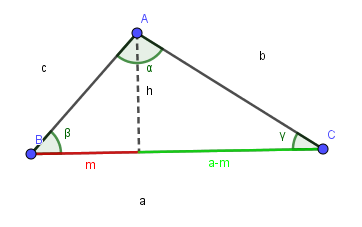
\includegraphics[width=0.6\linewidth]{triangulo.png}
		\end{center}
		\caption{Triângulo para ilustrar a lei dos cossenos.}
		\label{}
	\end{figure}
	É numa propriedade trigonométrica que é válida para qualquer triângulo, permitindo encontrar o valor de um lado do triângulo conhecendo apenas os outros lados e um ângulo. Porém, aqui utilizaremos a ideia reversa, porque, nesse caso, saberemos os lados e queremos descobrir os ângulos.
	
	\begin{itemize}
		\item \textbf{Demonstração Leis dos Cossenos:}
		
		Dado um triângulo qualquer, traça-se uma altura relativa ao lado $a$. Aplicando o \textit{Teorema de Pitágoras} no $\Delta ABC$:
		$$
		c^{2}=m^{2}+h^{2} \rightarrow h^{2}=c^{2}-m^{2}
		$$
		Aplicando novamente \textit{Pitágoras}, porém, em $\Delta ADC$, obtemos:
		$$
		b^{2}=h^{2}+(a-m)^{2}
		$$
		Substituindo nessa nova equação o valor de $h^{2}$ obtido:
		$$
		b^{2}=c^{2}-m^{2}+a^{2}-2am+m^{2}
		$$
		$$
		b^{2}=c^{2}+a^{2}-2m
		$$
		Podemos ver que $\frac{m}{b}=\cos\beta$, então:
		$$
		b^{2}=c^{2}+a^{2}-2ac\cos\beta
		$$
		Pode ser análogo também à:
		$$
		c^{2}=a^{2}+b^{2}-2ab\cos\gamma
		$$
		$$
		a^{2}=b^{2}+c^{2}-2bc\cos\alpha
		$$
		Podemos perceber que se o ângulo for $\frac{\pi}{2}$ recaímos no Teorema de Pitágoras. $\hfill\blacksquare$
		\item \textbf{Ângulos Entre 2 Vetores:}
		\begin{figure}[H]
			\begin{center}
				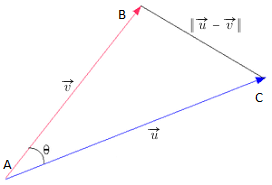
\includegraphics{Angulovetoresnovo.png}
			\end{center}
			\caption{Diferença entre vetores $u$ e $v$}
			\label{}
		\end{figure}
		Para encontrarmos a fórmula utilizaremos a lei dos cossenos aplicada a $\Delta ABC$:
		$$
		\|\overrightarrow{u}-\overrightarrow{v}\|^{2}=\|\overrightarrow{u}\|^{2} + \|\overrightarrow{v}\|^{2} - 2\|\overrightarrow{u}\|\|\overrightarrow{v}\|\cos\theta
		$$
		Utilizando propriedades do produto escalar
		$$
		\|\overrightarrow{u}-\overrightarrow{v}\|^{2}=\|\overrightarrow{u}\|^{2} + \|\overrightarrow{v}\|^{2} - 2\overrightarrow{u}\overrightarrow{v}
		$$
		Comparando as duas igualdades obtemos
		$$
		\|\overrightarrow{u}\|^{2} + \|\overrightarrow{v}\|^{2} - 2\|\overrightarrow{u}\|\|\overrightarrow{v}\|\cos\theta = \|\overrightarrow{u}\|^{2} + \|\overrightarrow{v}\|^{2} - 2\overrightarrow{u}\overrightarrow{v}
		$$
		$$
		\overrightarrow{u}\overrightarrow{v} = \|\overrightarrow{u}\|\|\overrightarrow{v}\|\cos\theta
		$$
		Logo,
		$$
		\cos\theta = \frac{\overrightarrow{u}\overrightarrow{v}}{\|\overrightarrow{u}\|\|\overrightarrow{v}\|} 
		$$
		$\hfill\blacksquare$
	\end{itemize}
	
	
\end{document}